\documentclass{article}

\usepackage{amsmath}
\usepackage{graphicx}

\addtolength{\oddsidemargin}{-.3in}
\addtolength{\evensidemargin}{-.3in}
\addtolength{\textwidth}{0.6in}

\begin{document}

\title{Homework 4\\
       N-body Assembly Line}
\author{Geoffrey Ulman\\
        CSI702}
\date{March 2010}
\maketitle

\section{Design}
My parallel N-body gravitational potential code uses the assembly line programming paradigm. Each node calculates the gravitational potential for \( \frac{n}{m} \) particles where \( n \) is the number of particles and \( m \) m is the number of nodes. These will be refered to as \emph{host particles}. In adition to the \( \frac{n}{m} \) host particles, each node has \( \frac{n}{m} \) \emph{guest particles}. The algorithm has \( n \) iterations.
During each iteration, the node calculates the gravitational potential between its host particles and guest particles then passes its guest particles to one of its neighbors while receiving another set of guest particles from its other neighbor. After each node has had the particles from all other nodes as guest particles, it reports its gravitational potential values back to node 0.

\section{Challenges}
Text...

\section{MPI Commands}
Like all MPI programs, the commands \verb!MPI_Init!, \verb!MPI_Comm_size!, \verb!MPI_Comm_rank!, and \verb!MPI_Finalize! were used to initialize and get basic information about the MPI environment. Because data was being passed in a ring, \verb!MPI_Cart_create! was used to create a new Cartesian comm group and \verb!MPI_Cart_shift! was used to determine the coordiates of the nodes neighbors. In addition, \verb!MPI_Cart_coords! was used to determine whether the node was in an even or odd positioin in the new Cartesian comm group. Data was sent using \verb!MPI_Isend! and \verb!MPI_Irecv! so that processing of the last group of host particles could be performed while the new group of host particles was being received. Finally, completion of the communications in each iteration was checked with \verb!MPI_Waitall!.

\section{Performance}
Text...

\begin{figure}
\centering
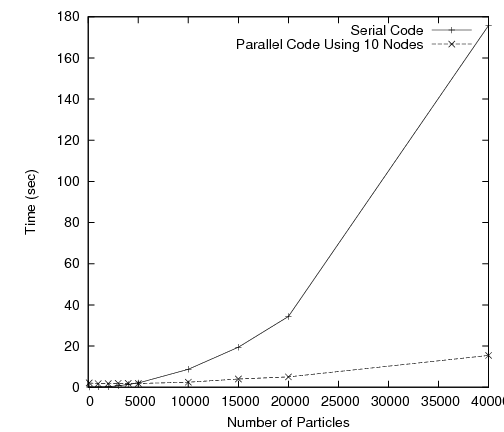
\includegraphics[width=0.6\textwidth]{img/timing_data_variable_particles.png}
\caption{Parallel and Serial Timing Results for Variable Particle Count}
\label{chart1}
\end{figure}

\begin{figure}
\centering
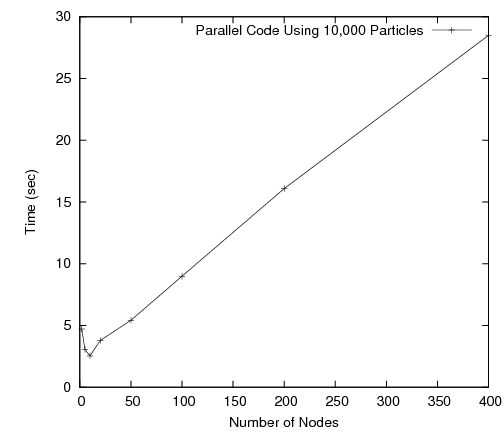
\includegraphics[width=0.6\textwidth]{img/timing_data_10000_particles.png}
\caption{Parallel and Serial Timing Results for 10,000 Particles}
\label{chart2}
\end{figure}

\begin{figure}
\centering
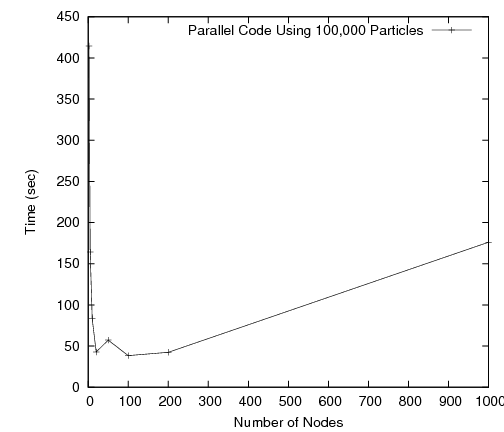
\includegraphics[width=0.6\textwidth]{img/timing_data_100000_particles.png}
\caption{Parallel and Serial Timing Results for 100,000 Particles}
\label{chart3}
\end{figure}

\section{Performance Comparison}
Text...

\section{Output Comparison}
The output of the serial and parallel codes are extrememly similar, however in most cases they were not identical. I used the \verb!MPI_FLOAT! data type to transfer data between nodes and c float to store them in the nodes. The error in the final calculation compared with the serial code was .

\begin{thebibliography}{9}

\bibitem{cpl}
  Brian W. Kernighan and Dennis M. Ritchie,
  \emph{The C Programming Language},
  Prentice Hall PTR, New Jersey,
  2009.

\end{thebibliography}

\end{document}
